% "Станет проще"

\documentclass[a4paper,12pt]{article} % тип документа

% report, book

%  Русский язык

\usepackage[T2A]{fontenc}			% кодировка
\usepackage[utf8]{inputenc}			% кодировка исходного текста
\usepackage{graphicx}
\usepackage[english,russian]{babel}	% локализация и переносы


%отступ
\usepackage[left=3cm,right=3cm,
    top=3cm,bottom=3cm,bindingoffset=0cm]{geometry}

% Математика
\usepackage{amsmath,amsfonts,amssymb,amsthm,mathtools} 
\usepackage{csvsimple}
\usepackage{multirow}

\usepackage{hyperref}
\usepackage{wasysym}
\usepackage{subcaption}
\usepackage{verbatim}
\usepackage{hyperref}
\usepackage{float}
\usepackage{enumerate}
\usepackage[dvipsnames]{xcolor}
%Заговолок
%\graphicspath{ {images/} }


\begin{titlepage}
\author{Соловьянов Михаил }
\title{Задание 7. Электродинамика.  Цепи с конденсаторами и катушками!}
\date{\today}
\end{titlepage}



\begin{document} % начало документа
\maketitle



\begin{figure}[H]
  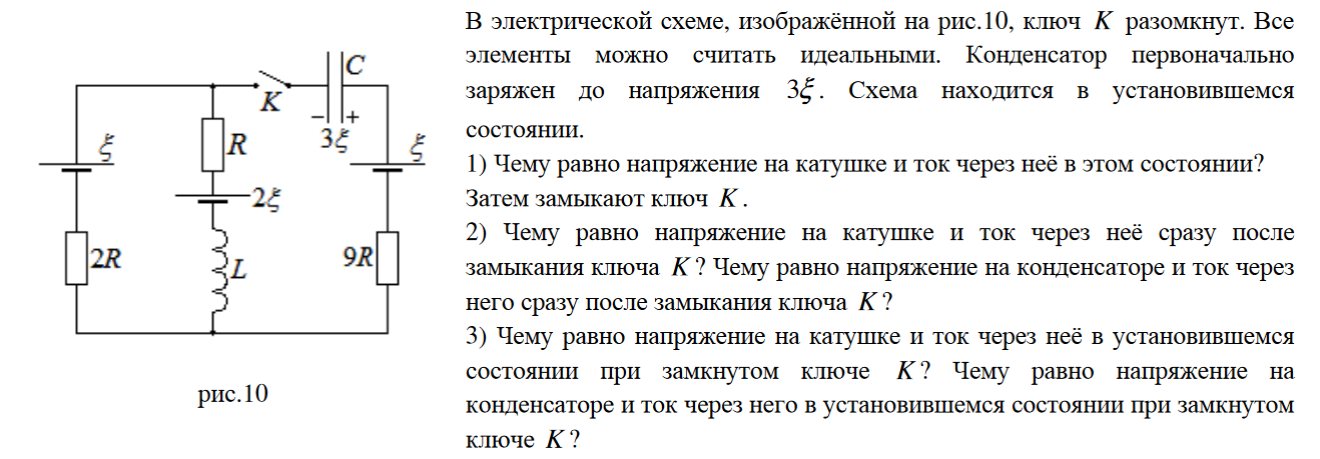
\includegraphics[width=\linewidth]{1.PNG}
  \caption{Задача 1 }
  \label{task1}
\end{figure}
 

\begin{figure}[H]
  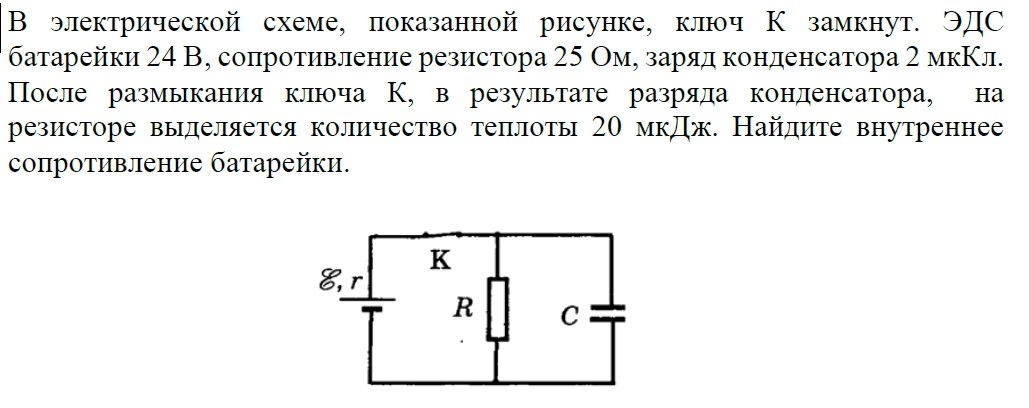
\includegraphics[width=\linewidth]{2.PNG}
  \caption{Задача 2 (из пробного ЕГЭ 2020 кстати) }
  \label{task2}
\end{figure}
 


\section{Контрольные вопросы}
\begin{enumerate}


\item Катушка индуктивности подключена в электрическую цепь. При каком условии сила тока, протекающего через катушку, меняется плавно?
\end{enumerate}


\section{Задачи}
\begin{enumerate}
\item Задача на рисунке, она же задача 2 из  \cite{l2} дорешать.


\item  Задача на рисунке  \ref{task2}  

\item  Задача 9 из \cite{l2}  

\item  Задача 10 из \cite{l2}  

\end{enumerate}

\section{Литература}
\begin{thebibliography}{}
    \bibitem{l1} СБОРНИК ОЛИМПИАДНЫХ ЗАДАЧ ПО ФИЗИКЕ Под редакцией Н.С. Кравченко
    \bibitem{l2} \url{https://vk.com/doc87612555_527254723?hash=54b73288a84f13bd56&dl=e2abb02099a4d83d46}
	
\end{thebibliography}



\end{document}